%----------------------------------------------------------------------------------------------------------------------%
% Author: John Joseph Valletta
% Date: 02/10/2015
% Title: A Gentle Introduction to Gaussian Processes
%----------------------------------------------------------------------------------------------------------------------%

%----------------------------------------------------------------------------------------------------------------------%
% Preamble
%----------------------------------------------------------------------------------------------------------------------%
\documentclass[pdf]{beamer}
\usepackage[export]{adjustbox}
\usepackage{framed}
\usepackage{color}
\usepackage{textpos} % textblock
\usepackage{blkarray} % To write on top/besides matrices
\usepackage{hyperref}
\hypersetup{colorlinks=true, urlcolor=blue, linkcolor=black} % For some reason it wasn't working when giving the parameters within the usepackage i.e \usepackage[]
\mode<presentation>{\usetheme{Madrid}} % default Antibes Berlin Madrid Montpelier Ilmenau CambridgeUS Berkeley Singapore Copenhagen Malmoe Warsaw
%\usecolortheme{dolphin}
%\definecolor{forestgreen}{rgb}{0.17, 0.67, 0.53} % (41, 171, 135)
%\definecolor{junglegreen}{rgb}{0.125, 0.5, 0.25}
\definecolor{tealblue}{rgb}{0, 0.5, 0.5}
\usecolortheme[named=tealblue]{structure}
\useinnertheme{circles} % circles, rectanges, rounded, inmargin
\usefonttheme[onlymath]{serif} % Makes math fonts like the usual LaTeX ones
%\useoutertheme{tree} % infolines, smoothbars, sidebar, split, tree
\setbeamercovered{transparent=4} % Transparent 10% overlays
\setbeamertemplate{caption}{\raggedright\insertcaption\par} % Remove the word "Figure" from caption %\setbeamertemplate{caption}[default]
\setbeamertemplate{navigation symbols}{} % don't put navigation tools at the bottom (alternatively \beamertemplatenavigationsymbolsempty)
\graphicspath{ {./Figures/} }
% Titlepage
\title[Introduction to Gaussian Processes]{A Gentle Introduction to Gaussian Processes}
\author{John Joseph Valletta}
\date[20th October 2015]{Internal Maths Seminar: 20th October 2015}
\institute[]{University of Exeter, Penryn Campus, UK}
\titlegraphic{
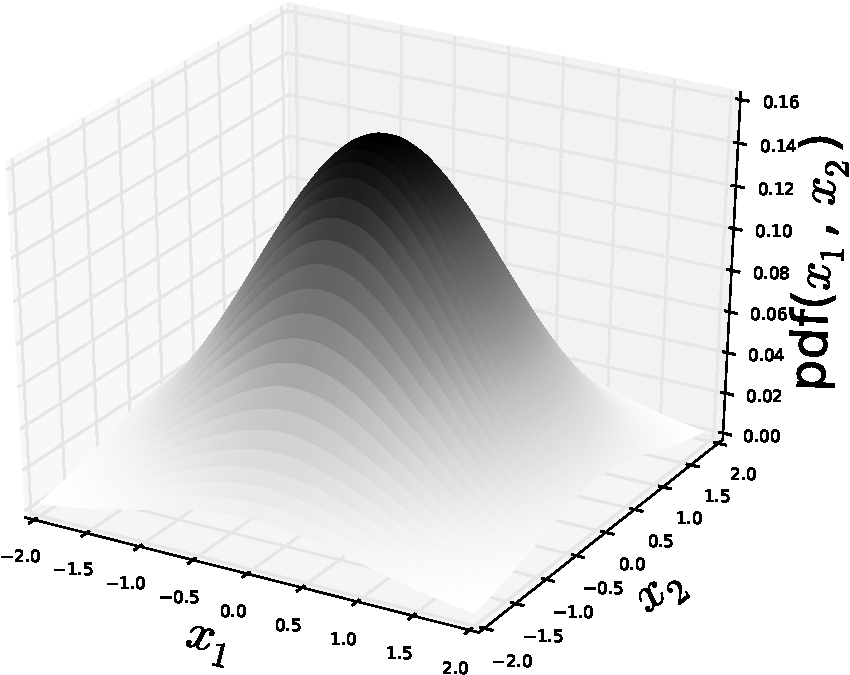
\includegraphics[width=0.35\textwidth, keepaspectratio]{Gaussian2D.pdf}
\hspace{1cm}
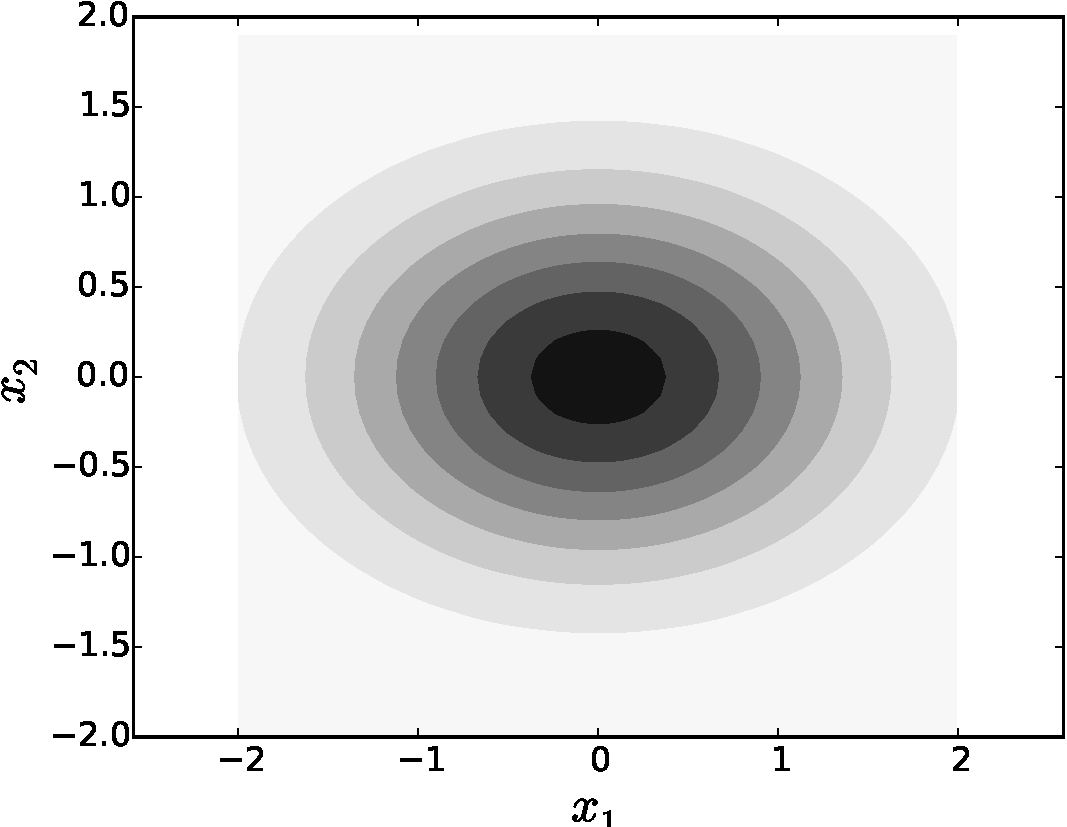
\includegraphics[width=0.35\textwidth, keepaspectratio]{Gaussian2DContour2.pdf}}

%----------------------------------------------------------------------------------------------------------------------%
% Start of Document
%----------------------------------------------------------------------------------------------------------------------%
\begin{document}

%----------------------------------------------------------------------------------------------------------------------%
%----------------------------------------------------------------------------------------------------------------------%
\begin{frame}
\titlepage
\end{frame}

%----------------------------------------------------------------------------------------------------------------------%
%----------------------------------------------------------------------------------------------------------------------%
\begin{frame}{Overview}
\begin{itemize}\addtolength{\itemsep}{0.5\baselineskip}
	\item<1-> Motivation	
 	\item<2-> The Gaussian Distribution
	\item<3-> Gaussian Processes
	\item<4-> Gaussian Process Regression - A Toy Example
	\item<5-> Gaussian Process Regression - CO$_2$ Concentrations 
	\item<6-> Modelling Gene Expression Time-Series
\end{itemize}
\end{frame}

%----------------------------------------------------------------------------------------------------------------------%
%----------------------------------------------------------------------------------------------------------------------%
\begin{frame}{Motivation}
\begin{center}
	\includegraphics<1>[width=0.8\textwidth]{CO2Raw.pdf}
	\includegraphics<2>[width=0.8\textwidth]{CO2PolyFit1.pdf}
	\includegraphics<3>[width=0.8\textwidth]{CO2PolyFit2.pdf}
\end{center}
\end{frame}

%----------------------------------------------------------------------------------------------------------------------%
%----------------------------------------------------------------------------------------------------------------------%
\begin{frame}{The Data Modelling Task}
\begin{itemize}\addtolength{\itemsep}{1\baselineskip}
	\item \textbf{data}: $\mathbf{x} = \{x_1,\ldots, x_N\}$, $\mathbf{y} = \{y_1,\ldots, y_N\}$
	\item \textbf{model}: $y = f(x) + \epsilon$\\
	\item \textbf{predictions}: $y^* = f(x^*)$
\end{itemize}
\begin{center}
	\visible<2>{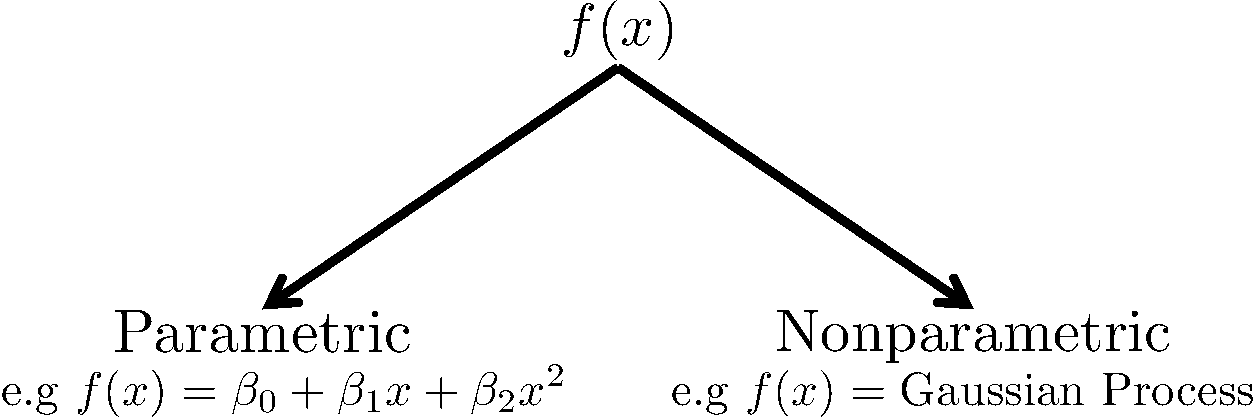
\includegraphics[width=0.9\textwidth]{ModelType.pdf}}
\end{center}
\end{frame}

%----------------------------------------------------------------------------------------------------------------------%
%----------------------------------------------------------------------------------------------------------------------%
\begin{frame}{The Gaussian Distribution}
\begin{center}
	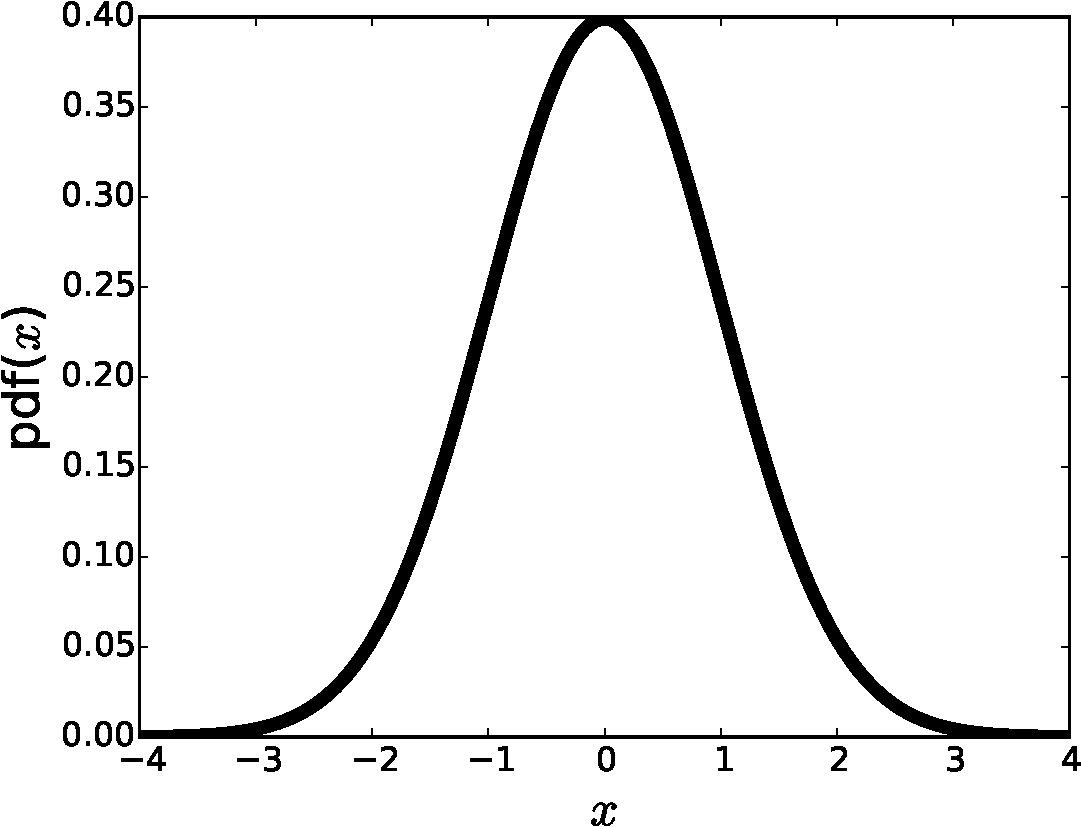
\includegraphics[width=0.5\textwidth]{Gaussian1D.pdf}
	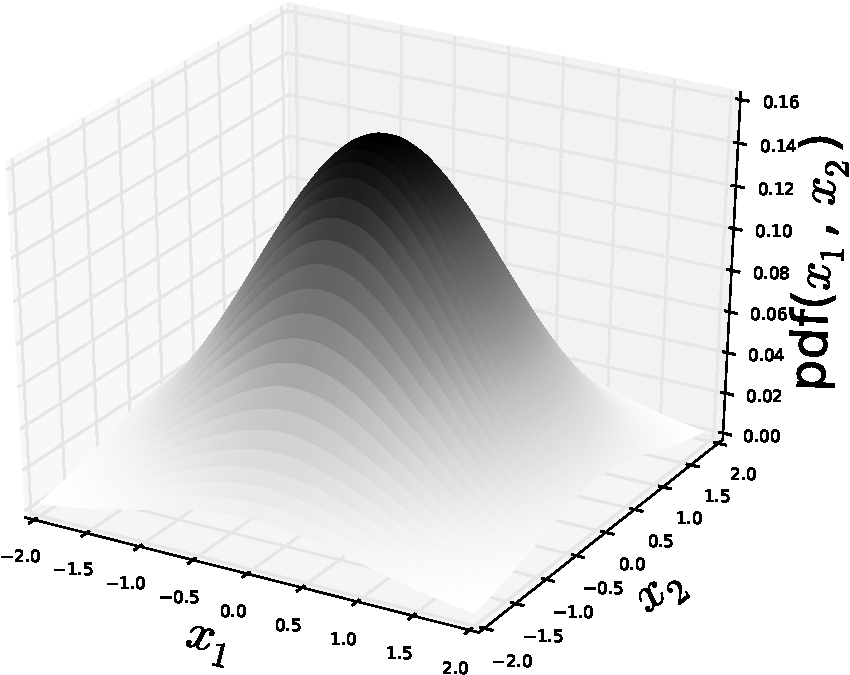
\includegraphics[width=0.5\textwidth]{Gaussian2D.pdf}
\end{center}

\begin{textblock}{8}(3, 0) %{width}(x position, y position) (0, 0) is top left corner 
% Default unit is 1/16 of paper height and paper width
$\mathcal{N}(\mu,\ \sigma^2)$
\end{textblock}

\begin{textblock}{8}(0, 1.5) %{width}(x position, y position) (0, 0) is top left corner 
% Default unit is 1/16 of paper height and paper width
\scriptsize
A draw from this distribution is a 1D vector\\
e.g $x=[0.2]$
\end{textblock}

\begin{textblock}{8}(10, 0) %{width}(x position, y position) (0, 0) is top left corner 
% Default unit is 1/16 of paper height and paper width
$\mathcal{N}(\boldsymbol{\mu},\ \Sigma)$
\end{textblock}

\begin{textblock}{8}(8, 1.5) %{width}(x position, y position) (0, 0) is top left corner 
% Default unit is 1/16 of paper height and paper width
\scriptsize
A draw from this distribution is a 2D vector\\
e.g $\mathbf{x}=\begin{bmatrix} 0.3 \\ -0.4 \end{bmatrix}$
\end{textblock}

\begin{center} % If I delete this I'd have to reposition "textblock" so leave it as it until next time
\end{center}
\end{frame}

%----------------------------------------------------------------------------------------------------------------------%
%----------------------------------------------------------------------------------------------------------------------%
\begin{frame}{The Covariance Matrix}
\begin{center}
	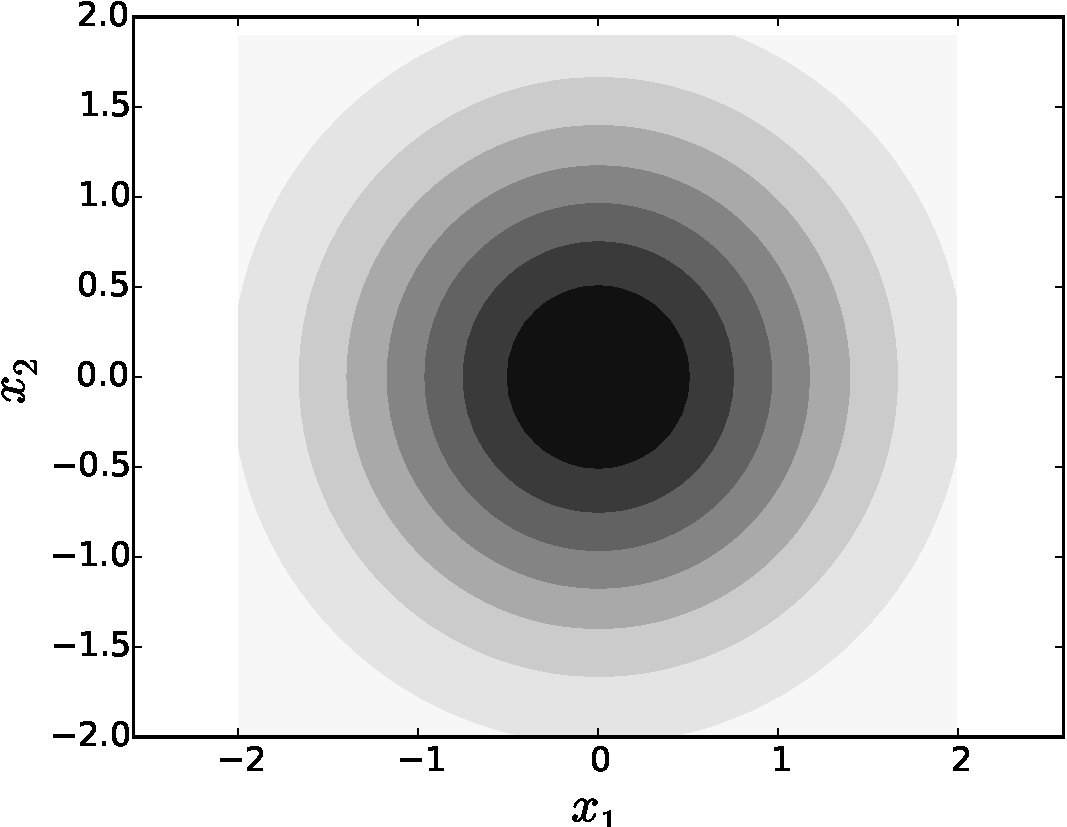
\includegraphics[width=0.5\textwidth]{Gaussian2DContour1.pdf}
	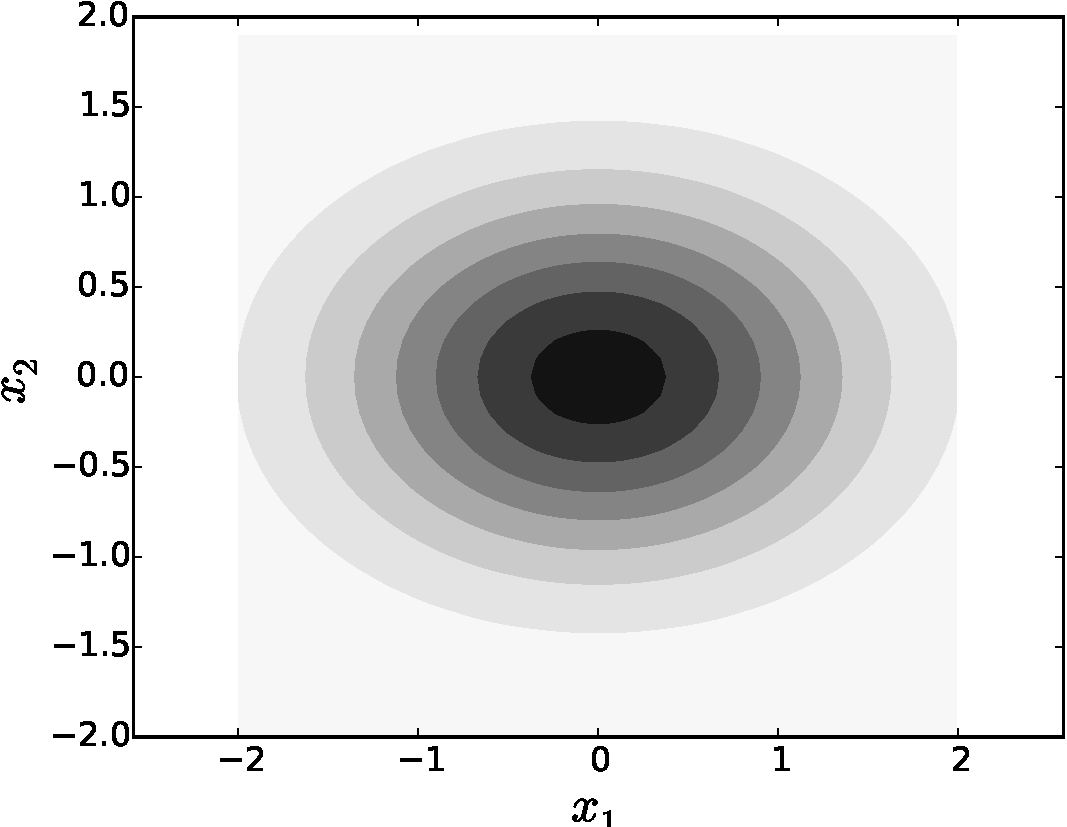
\includegraphics[width=0.5\textwidth]{Gaussian2DContour2.pdf}
\end{center}

\begin{textblock}{8}(3.2, 0) %{width}(x position, y position) (0, 0) is top left corner 
% Default unit is 1/16 of paper height and paper width
\textbf{Isotropic}
\end{textblock}

\begin{textblock}{8}(3, 1.5) %{width}(x position, y position) (0, 0) is top left corner 
% Default unit is 1/16 of paper height and paper width
$\Sigma = 
\begin{pmatrix}
1 & 0\\
0 & 1
\end{pmatrix}
$
\end{textblock}

\begin{textblock}{8}(10.5, 0) %{width}(x position, y position) (0, 0) is top left corner 
% Default unit is 1/16 of paper height and paper width
\textbf{Diagonal}
\end{textblock}

\begin{textblock}{8}(10, 1.5) %{width}(x position, y position) (0, 0) is top left corner 
% Default unit is 1/16 of paper height and paper width
$\Sigma = 
\begin{pmatrix}
1 & 0\\
0 & 0.5
\end{pmatrix}
$
\end{textblock}

\begin{center}
\end{center}
\end{frame}

%----------------------------------------------------------------------------------------------------------------------%
%----------------------------------------------------------------------------------------------------------------------%
\begin{frame}{The Covariance Matrix}
\begin{center}
	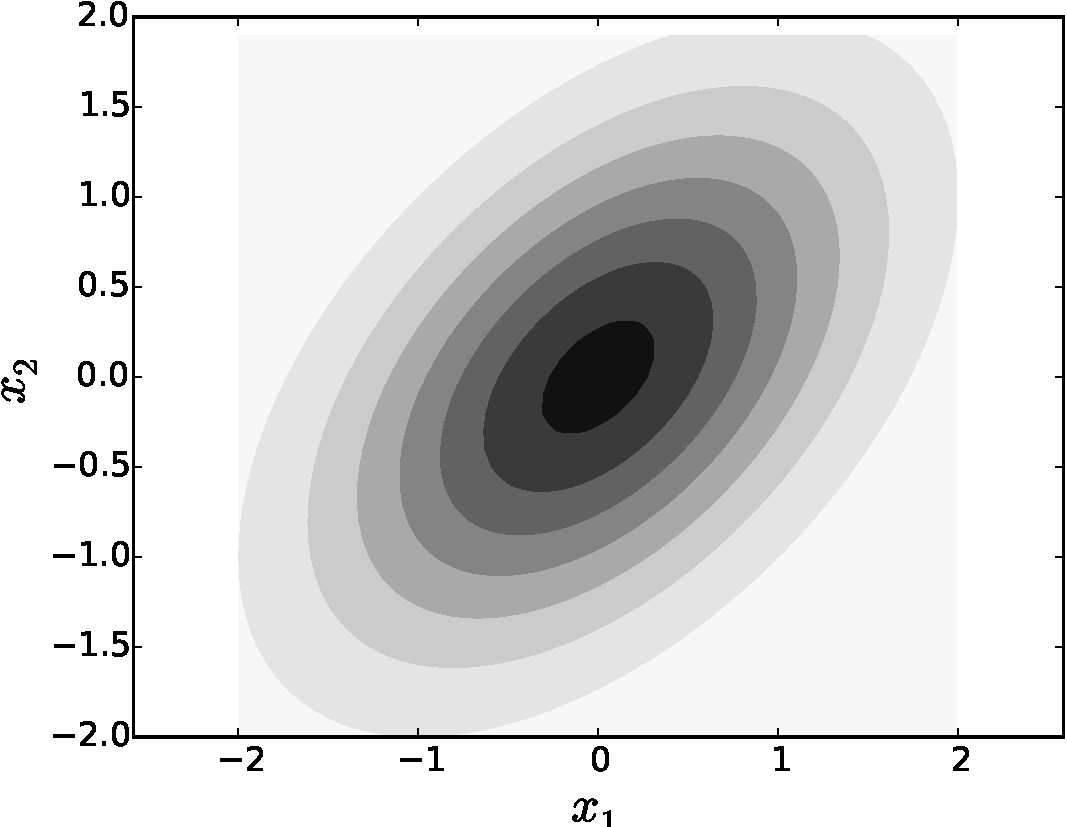
\includegraphics[width=0.5\textwidth]{Gaussian2DContour3.pdf}
	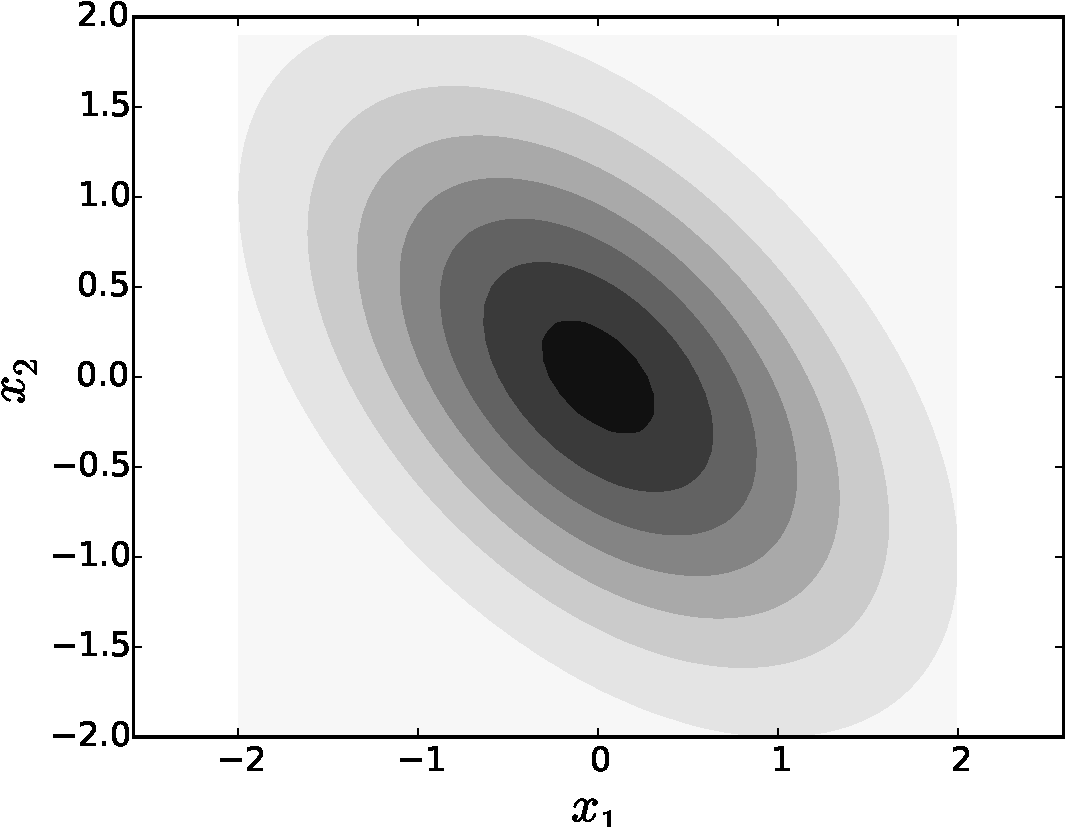
\includegraphics[width=0.5\textwidth]{Gaussian2DContour4.pdf}
\end{center}

\begin{textblock}{8}(2.6, 0) %{width}(x position, y position) (0, 0) is top left corner 
% Default unit is 1/16 of paper height and paper width
\textbf{General Form}
\end{textblock}

\begin{textblock}{8}(2.4, 1.5) %{width}(x position, y position) (0, 0) is top left corner 
% Default unit is 1/16 of paper height and paper width
$\Sigma = 
\begin{pmatrix}
1 & 0.5\\
0.5 & 1
\end{pmatrix}
$
\end{textblock}

\begin{textblock}{8}(10.2, 0) %{width}(x position, y position) (0, 0) is top left corner 
% Default unit is 1/16 of paper height and paper width
\textbf{General Form}
\end{textblock}

\begin{textblock}{8}(9.8, 1.5) %{width}(x position, y position) (0, 0) is top left corner 
% Default unit is 1/16 of paper height and paper width
$\Sigma = 
\begin{pmatrix}
1 & -0.5\\
-0.5 & 1
\end{pmatrix}
$
\end{textblock}

\begin{center}
\end{center}
\end{frame}

%----------------------------------------------------------------------------------------------------------------------%
%----------------------------------------------------------------------------------------------------------------------%
\begin{frame}{Sampling from a Multivariate Gaussian}
What does a \textit{single} sample from a 100 dimensional Gaussian look like?
\vspace{1cm}
\begin{columns}
\column{0.45\textwidth}
	$\mathbf{x}=
	\left[
	\begin{array}{c}
	0.2 \\ \vdots \\ \vdots \\ \vdots \\ \vdots \\ \vdots \\ \vdots \\ -0.6
	\end{array}
	\right]
	\left.
	\begin{array}{c}
	 \\  \\  \\  \\  \\  \\  \\ \\  \\ \\ \\ % maybe there's a better way to do this but don't know
	\end{array}
	\right\}
	\begin{array}{c}
	 \\  \\  \\  \\ \\ =100 \Longrightarrow \\  \\ \\  \\ \\ \\ % maybe there's a better way to do this but don't know
	\end{array}
	$
\column{0.55\textwidth}
\begin{center}
	\visible<2>{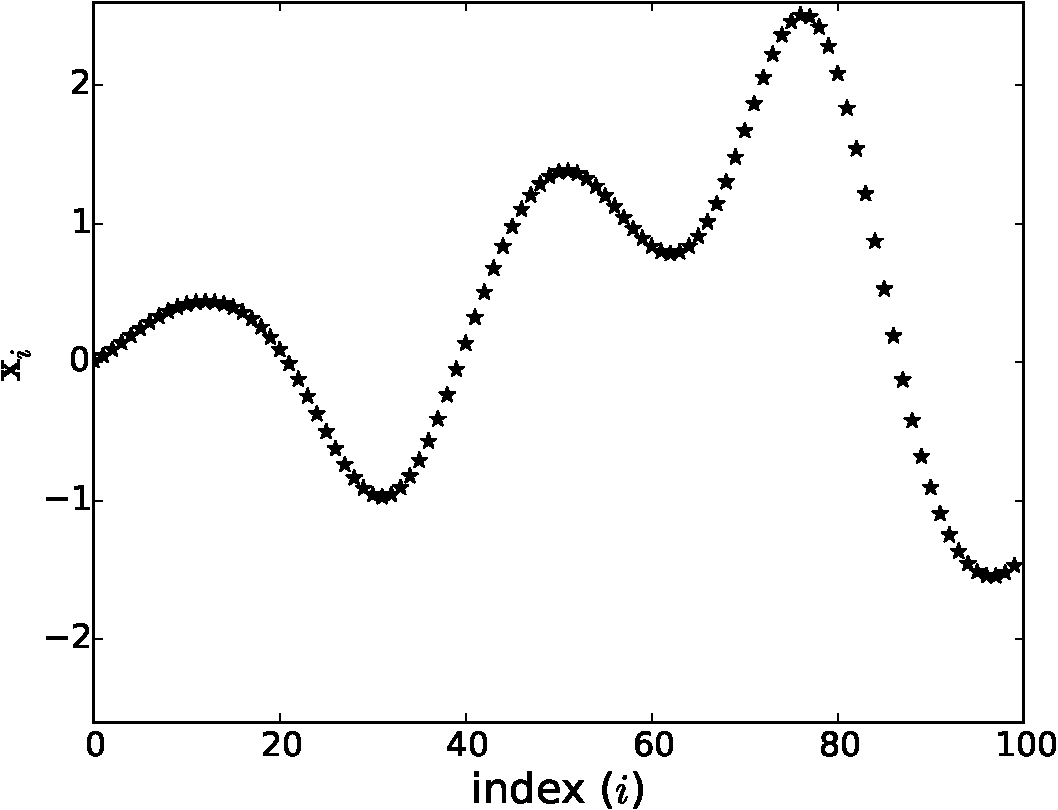
\includegraphics[width=\textwidth]{Gaussian100D.pdf}}
\end{center}
\end{columns}
\end{frame}

%----------------------------------------------------------------------------------------------------------------------%
%----------------------------------------------------------------------------------------------------------------------%
\begin{frame}{Gaussian Process in a Nutshell}
\vspace{-0.2cm}
\textbf{Recall}: What we are after is $y = f(x)$\\
\vspace{0.3cm}
\textbf{Trick}: Think about a function as an infinitely-long vector 
%specifying the value of the function at a particular input (x)
\begin{columns}
\column{0.51\textwidth}
	$f(x) =
	\left[
	\begin{array}{c}
	f_1 \\ \vdots \\ \vdots \\ \vdots \\ \vdots \\ \vdots \\ \vdots \\ f_\infty
	\end{array}
	\right]
	\left.
	\begin{array}{c}
	 \\  \\  \\  \\  \\  \\  \\ \\  \\ \\ \\ % maybe there's a better way to do this but don't know
	\end{array}
	\right\}
	\begin{array}{c}
	 \\  \\  \\  \\ \\ =\infty \Longrightarrow \\  \\ \\  \\ \\ \\ % maybe there's a better way to do this but don't know
	\end{array}
	$
\column{0.49\textwidth}
\begin{center}
	\visible<2->{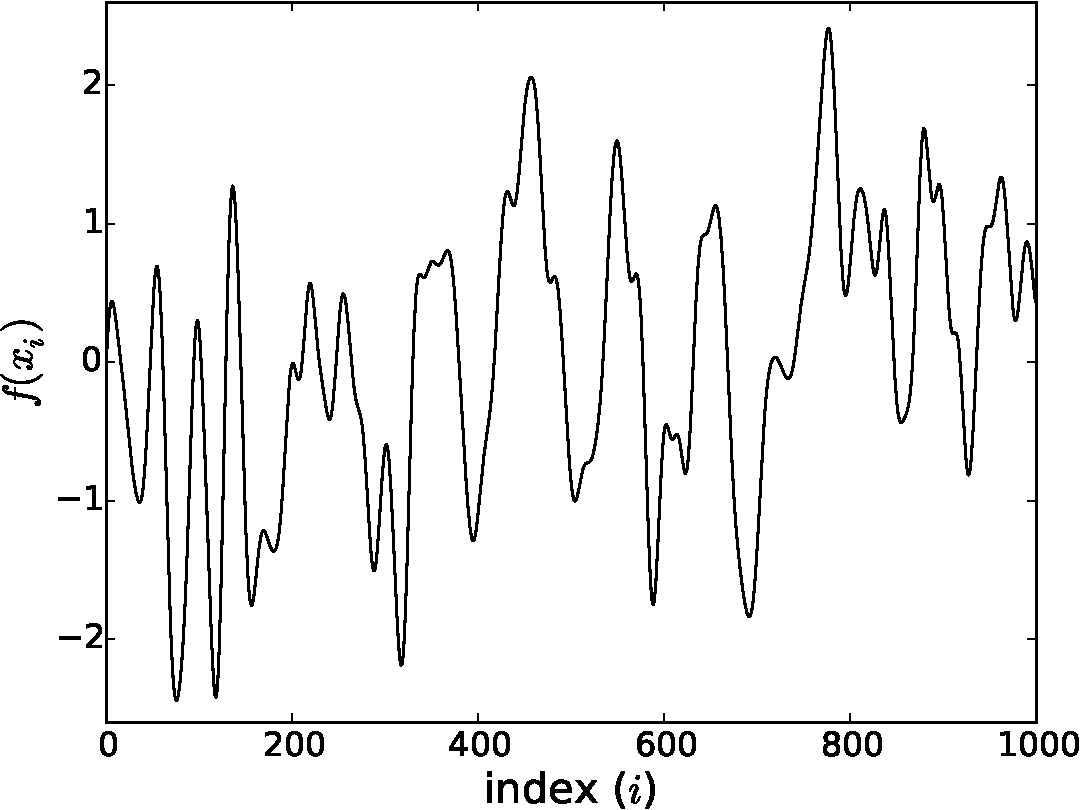
\includegraphics[width=\textwidth]{GaussianInfD.pdf}}
\end{center}
\end{columns}
\vspace{0.25cm}
\visible<3->{\textbf{Computational Madness}: Ask only for the properties of the function at a \textit{finite} number of points}
\end{frame}

%----------------------------------------------------------------------------------------------------------------------%
%----------------------------------------------------------------------------------------------------------------------%
\begin{frame}{Gaussian Process in a Nutshell}
\small
\begin{columns}
% 3D Gaussian
\column{0.42\textwidth}
\begin{block}{3 dimensional Gaussian}
% Mean vector
Mean vector
\\[0.2cm]
$\mu = 
\begin{pmatrix}
\mu_1 \\ \\ \mu_2 \\ \\ \mu_3
\end{pmatrix}
$
\\[0.6cm]
% Covariance function
Covariance matrix
\\[0.4cm]
$\Sigma = 
\begin{pmatrix}
  	\sigma^2_1 & & \sigma_{12} & & \sigma_{13}\\
  	& & & & \\	
  	\sigma_{21} & & \sigma^2_2 & & \sigma_{23} \\
	& & & & \\
	\sigma_{31} & & \sigma_{32} & & \sigma^2_3 \\
\end{pmatrix}
$
\end{block}

% Infinite Gaussian
\column{0.56\textwidth}
\begin{block}{$\infty$ dimensional Gaussian}
% Mean vector
Mean \textit{function}
\\[0.2cm]
$\mu = 
\begin{pmatrix}
\mu_1 \\ \vdots \\ \vdots \\ \mu_\infty
\end{pmatrix}
= m(\mathbf{x})
$
\\[0.5cm]
% Covariance function
Covariance \textit{function}
\\[0.2cm]
$\Sigma = 
\begin{pmatrix}
  	\sigma^2_1 		& \sigma_{12}  		& \hdots & \sigma_{1\infty}\\
  	\sigma_{21}		& \sigma^2_2 		& \hdots & \vdots \\
	\vdots 			& \vdots 			& \ddots & \vdots \\
	\vdots 			& \vdots 			& \hdots & \sigma^2_\infty
\end{pmatrix}
= k(\mathbf{x},\mathbf{x}')
$
\end{block}

\end{columns}

\end{frame}
% \[\Sigma =
% \begin{blockarray}{cccc}
% & x_1 & x_2 & x_3 \\
% \begin{block}{c(ccc)}
%   x_1 & \sigma^2_{x_1} & \sigma_{x_1}\sigma_{x_2} & \sigma_{x_1}\sigma_{x_3}\\
%   x_2 & \sigma_{x_2}\sigma_{x_1} & \sigma^2_{x_2} & \sigma_{x_2}\sigma_{x_3} \\
%   x_3 & \sigma_{x_3}\sigma_{x_1} & \sigma_{x_3}\sigma_{x_2} & \sigma^2_{x_3} \\
% \end{block}
% \end{blockarray}
% \]

%----------------------------------------------------------------------------------------------------------------------%
%----------------------------------------------------------------------------------------------------------------------%
\begin{frame}{Gaussian Process}

\begin{block}{Definition}
A Gaussian Process (GP) is an infinite collection of random variables, any finite number of which have a joint normal distribution.
\\
Essentially an infinite dimension multivariate Gaussian distribution, characterised by a mean function $m(\mathbf{x})$ and a covariance function $k(\mathbf{x},\mathbf{x}')$ 
\end{block}

\begin{block}{Rationale}
Instead of inferring the parameters of a fixed model structure ($\beta_0,\beta_1,\ldots$), with GPs we model the \textit{correlation}
between inputs. That is, inputs $\mathbf{x}$ that are close/similar to each other are likely to give rise to a similar
output $f(\mathbf{x})$  
\end{block}
\vspace{-1cm}
\begin{align}
f(\mathbf{x})\ \ \sim\ \ &\mathrm{GP}(m(\mathbf{x}),k(\mathbf{x},\mathbf{x}'))\nonumber\\
m(\mathbf{x})\ \ =\ \ &\mathrm{E}[f(\mathbf{x})]\nonumber\\
k(\mathbf{x},\mathbf{x}')\ \ =\ \ &\mathrm{E}[(f(\mathbf{x})-m(\mathbf{x})(f(\mathbf{x}')-m(\mathbf{x}')]\nonumber
\end{align} 

\end{frame}

%----------------------------------------------------------------------------------------------------------------------%
%----------------------------------------------------------------------------------------------------------------------%
\begin{frame}{Covariance Function}
\begin{itemize}\addtolength{\itemsep}{0.2\baselineskip}
	\item<1-> Vital ingredient in Gaussian Process\footnote{without much loss of generality we can assume that $m(\mathbf{x}) \equiv 0$} 
	\item<2-> Encodes our assumptions about the function we wish to model (smooth, stationary, etc.)
	\item<3-> Quantifies the \textit{similarity} between two data points; crucial for predicting a test point $\mathbf{x^*}$
	\item<4-> Needs to satisfy a set of mathematical conditions {\tiny (beyond the scope of this intro)}
	\item<5-> A very popular choice is the Squared Exponential:\\ 
	{\tiny (also known as RBF, Gaussian and Exponentiated Quadratic Kernel Function)} 
	$$
	k(\mathbf{x},\mathbf{x}') = \alpha \exp \left( {\frac{\Vert \mathbf{x} - \mathbf{x'} \Vert^2}{2l^2}} \right)
	$$
	e.g if we set $\alpha=1$ and $l=1$ then:\\
 	{\footnotesize $k(0, 0) = e^0 = 1$,\ \ \ \ \ $k(0, 1) = e^{-\frac{1}{2}} = 0.6$,\ \ \ \ \ $k(0, 2) = e^{-2} = 0.14$}
\end{itemize}
\end{frame}

%----------------------------------------------------------------------------------------------------------------------%
%----------------------------------------------------------------------------------------------------------------------%
\begin{frame}{Gaussian Process Regression}
\begin{itemize}\addtolength{\itemsep}{1\baselineskip}
	\item<1-> Shift the problem from inferring model parameters to choosing a covariance function and its (hyper)parameters
	\item<2-> Choose $m(\mathbf{x})$ and $k(\mathbf{x},\mathbf{x}')$ that reflect some prior belief
	\item<3-> This defines a \textit{prior} on the function class itself; it is a prior on a \textit{function} and not 
	parameters of some fixed model structure
	\item<4-> Under a Bayesian framework this prior is ``reshaped'' by the observed data to obtain a posterior distribution
	on the \textit{function}
\end{itemize}
\end{frame}

%----------------------------------------------------------------------------------------------------------------------%
%----------------------------------------------------------------------------------------------------------------------%
\begin{frame}{Gaussian Process Regression - A Toy Example}
\begin{center}
	\includegraphics<1>[width=0.85\textwidth]{GPPrior.pdf}
	\includegraphics<2>[width=0.85\textwidth]{GP0Point.pdf}
	\includegraphics<3>[width=0.85\textwidth]{GP1Point.pdf}
	\includegraphics<4>[width=0.85\textwidth]{GP2Point.pdf}
	\includegraphics<5>[width=0.85\textwidth]{GP5Point.pdf}
	\includegraphics<6>[width=0.85\textwidth]{GP11Point.pdf}
	\includegraphics<7>[width=0.85\textwidth]{GP23Point.pdf}
	\includegraphics<8>[width=0.85\textwidth]{GP39Point.pdf}
\end{center}
\end{frame}

%----------------------------------------------------------------------------------------------------------------------%
%----------------------------------------------------------------------------------------------------------------------%
\begin{frame}{Misspecifying the Covariance Function}
\begin{itemize}\addtolength{\itemsep}{0.5\baselineskip}
	\item<1-> The Squared Exponential covariance function was used in the previous example:
	$$
	k(\mathbf{x},\mathbf{x}') = \alpha \exp \left( {\frac{\Vert \mathbf{x} - \mathbf{x'} \Vert^2}{2l^2}} \right)
	$$
	\item<2-> Choosing a covariance functions is akin to choosing a model structure; it dictates the class of functions
	that can be represented by the Gaussian Process\footnote{typically a wider class of functions than in parametric models}
 	\item<3-> Misspecifying the covariance function and/or its (hyper)parameters has a detrimental effect on the model fit
 	\item<4-> For e.g in the squared exponential case the lengthscale $l$ dictates how much the function is allowed to bend 
\end{itemize}
\end{frame}

%----------------------------------------------------------------------------------------------------------------------%
%----------------------------------------------------------------------------------------------------------------------%
\begin{frame}{The Effect of Lengthscale on Model Fit}
\begin{center}
	\includegraphics<1>[width=0.83\textwidth]{GPLengthscale0.pdf}
	\includegraphics<2>[width=0.83\textwidth]{GPLengthscale1.pdf}
	\includegraphics<3>[width=0.83\textwidth]{GPLengthscale2.pdf}
	\includegraphics<4>[width=0.83\textwidth]{GPLengthscale3.pdf}
	\includegraphics<5>[width=0.83\textwidth]{GPLengthscale4.pdf}
	\includegraphics<6>[width=0.83\textwidth]{GPLengthscale5.pdf}
	\includegraphics<7>[width=0.83\textwidth]{GPLengthscale6.pdf}
	\includegraphics<8>[width=0.83\textwidth]{GPLengthscale7.pdf}
	%\includegraphics<9>[width=0.85\textwidth]{GPLengthscale8.pdf}
\end{center}
\end{frame}

%----------------------------------------------------------------------------------------------------------------------%
%----------------------------------------------------------------------------------------------------------------------%
\begin{frame}{Learning the Covariance Parameters}
\begin{itemize}\addtolength{\itemsep}{0.5\baselineskip}
	\item<1-> Let us define $\theta$ as a vector containing all (hyper)parameters \\
	e.g $\theta = \{\alpha, l, \sigma^2_n\}$
	\item<2-> We choose $\theta$ that maximises the log marginal likelihood, that is:
	%\mathrm{argmax}_{\mathbf{\theta}\in\mathbb{R}^D} 
$$
\ln p(y|\mathbf{x},\mathbf{\theta})=-\frac{1}{2}y^T(k(\mathbf{x},\mathbf{x}')+\sigma^2_nI)^{-1}y-\frac{1}{2}\ln|k(\mathbf{x},\mathbf{x}')+\sigma^2_nI|-\frac{n}{2}\ln2\pi
$$
	\item<3-> Cannot guarantee a global optimum; try different initial conditions
	\item<4-> Constraint (hyper)parameters to some sensible limits
	\item<5-> \textbf{Note}: Choosing the right covariance function (e.g Squared Exponential, Mat\'{e}rn, Rational Quadratic, etc.) is not always easy and
	should be treated akin to a model selection problem
\end{itemize}
\end{frame}

%----------------------------------------------------------------------------------------------------------------------%
%----------------------------------------------------------------------------------------------------------------------%
\begin{frame}{Modelling CO$_2$ Concentrations}
\begin{center}
	\includegraphics<1>[width=\textwidth]{CO2RawTake2.pdf}
	\includegraphics<2>[width=\textwidth]{CO2GPFit.pdf}
\end{center}
\end{frame}

%----------------------------------------------------------------------------------------------------------------------%
%----------------------------------------------------------------------------------------------------------------------%
\begin{frame}{Modelling Gene Expression Time-Series}
\begin{center}
	\includegraphics<1>[width=0.8\textwidth]{ProbeRaw.pdf}
	\includegraphics<2>[width=0.8\textwidth]{ProbeGP.pdf}
	\includegraphics<3>[width=0.8\textwidth]{ProbeGPAnnotate.pdf}
\end{center}
\end{frame}

%----------------------------------------------------------------------------------------------------------------------%
%----------------------------------------------------------------------------------------------------------------------%
\begin{frame}{Ranking Gene Expression Time-Series}
\begin{center}
	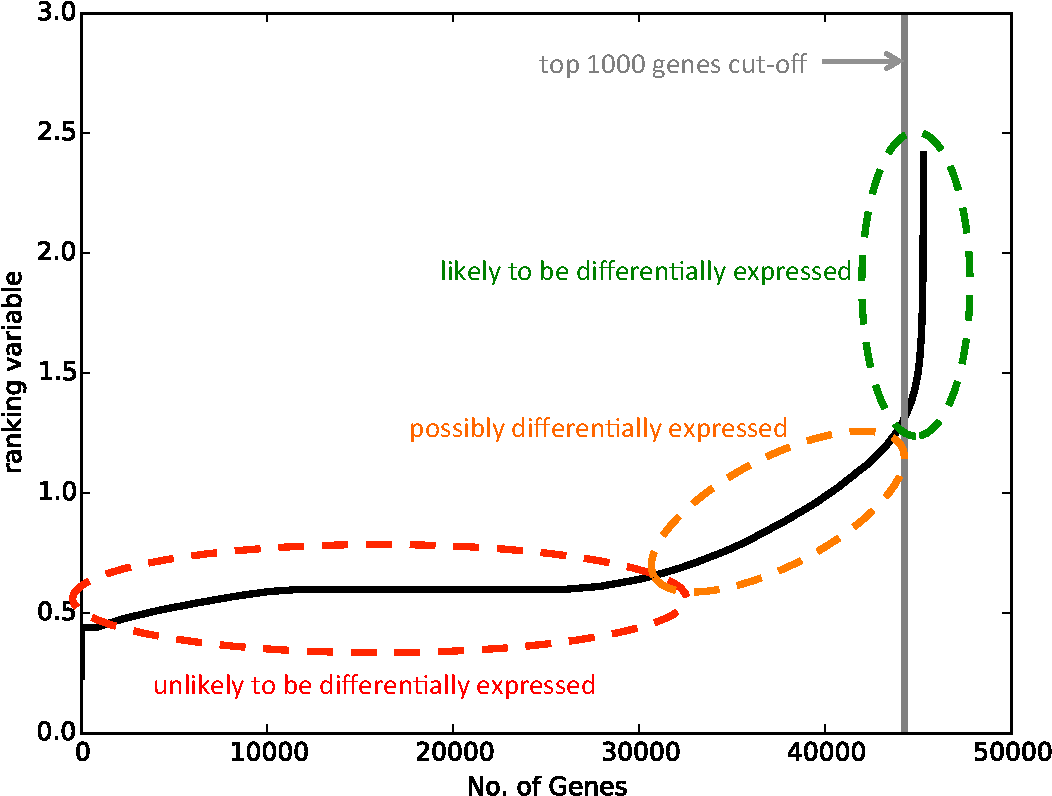
\includegraphics[width=0.85\textwidth]{ProbeRanking.pdf}
\end{center}
\end{frame}

%----------------------------------------------------------------------------------------------------------------------%
%----------------------------------------------------------------------------------------------------------------------%
\begin{frame}{Clustering Gene Expression Time-Series}
\begin{center}
	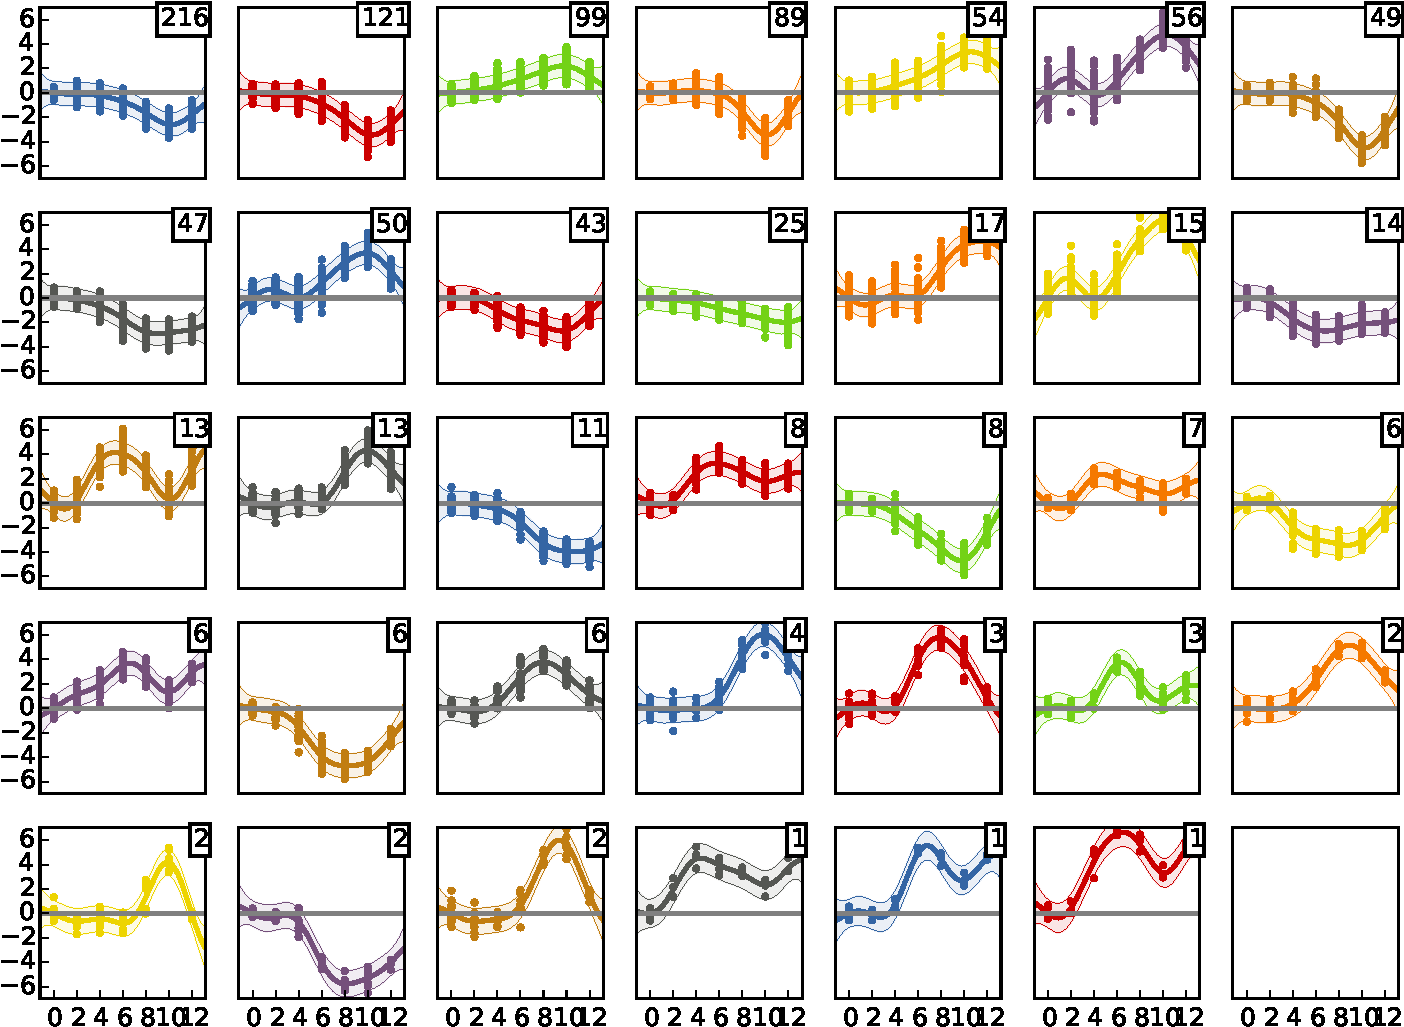
\includegraphics[width=0.9\textwidth]{ProbeClustering.pdf}
\end{center}
\end{frame}

%----------------------------------------------------------------------------------------------------------------------%
%----------------------------------------------------------------------------------------------------------------------%
\begin{frame}{Gaussian Process Resources}
\begin{itemize}\addtolength{\itemsep}{0.3\baselineskip}
	\item Rasmussen and Williams book
	\begin{center}
		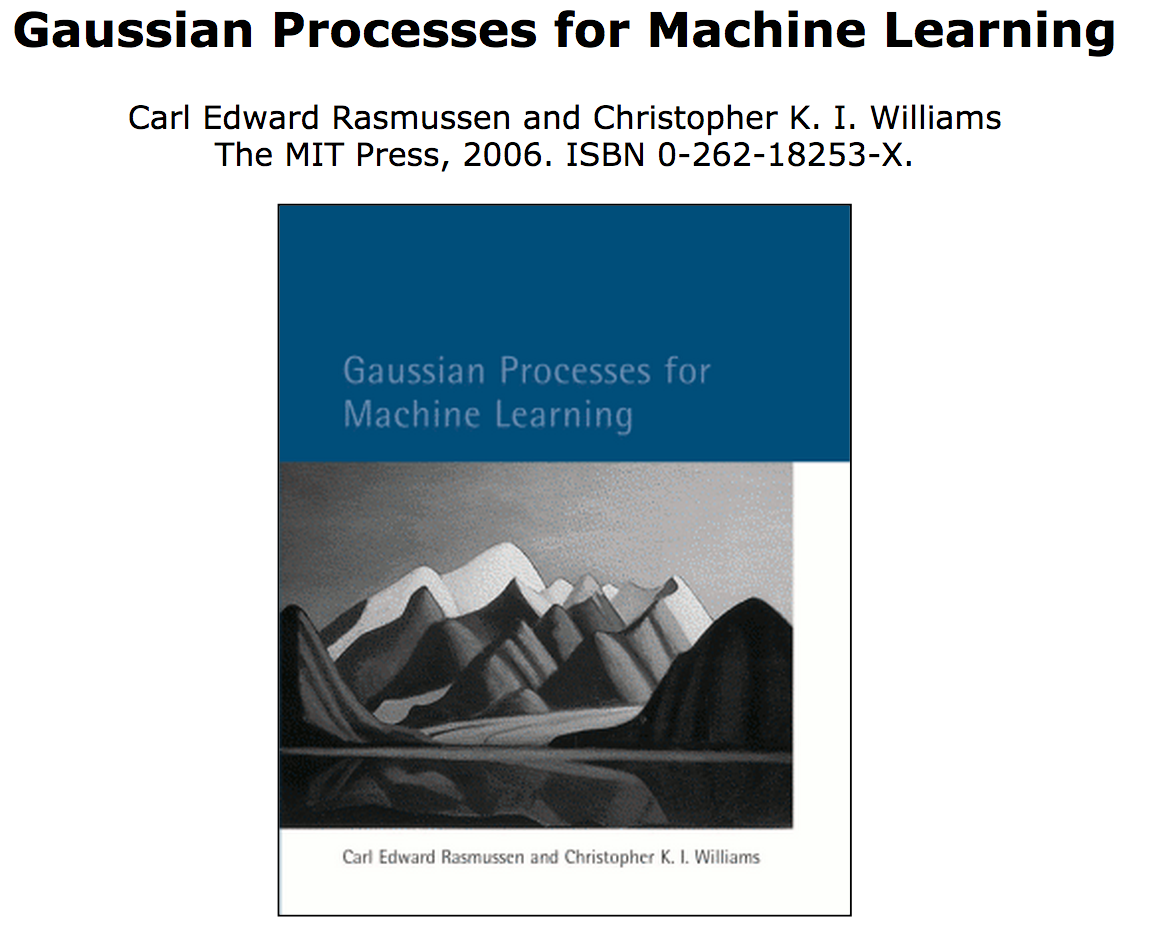
\includegraphics[width=0.5\textwidth]{GPBook.png}
	\end{center}
	\item \href{http://www.gaussianprocess.org/}{http://www.gaussianprocess.org/}
	\item The \texttt{GPy} Python Module by Neil Lawrence's Sheffield Group:\\ 
	\href{https://github.com/SheffieldML/GPy}{https://github.com/SheffieldML/GPy}
\end{itemize}
\end{frame}

%-------------------------------------------------------------------------------------------------%
% End of Document
%-------------------------------------------------------------------------------------------------%
\end{document}
